% !TEX program = lualatex
% George Mason University dissertation or thesis, 2027 UDTS accessible template,
% manuscript configuration with a reference list at the end of each chapter.
% Compile with LuaLaTeX (TeX Live 2026). On Overleaf: Menu > Compiler: LuaLaTeX,
% TeX Live version: 2026, Main document: main.tex.
%
% Edit these files for your own document:
%   frontmatter/metadata.tex      title, your name, degree, committee, signature lines
%   frontmatter/*.tex             dedication, acknowledgments, lists, abstract, biography
%   chapters/*.tex                your chapters, each ending with \chapterreferences
%   references.bib                your bibliography
% Leave gmuETD.sty unchanged. Options that change its output are in preamble/overrides.tex.
% UDTS requires the accessible template for the Spring 2027 degree term.
% MathML for the mathematics is produced by LuaLaTeX. pdfLaTeX tags the
% document and attaches the LaTeX source of each formula instead.
\ifdefined\directlua
  \DocumentMetadata{
    lang=en,
    pdfstandard=ua-2,
    tagging=on,
    tagging-setup={math/setup=mathml-SE}
  }
\else
  \DocumentMetadata{
    lang=en,
    pdfstandard=ua-2,
    tagging=on
  }
\fi
% These are the paragraph socket settings supplied by the UDTS template.
\AssignTaggingSocketPlug{para/semantic/begin}{noop}
\AssignTaggingSocketPlug{para/semantic/end}{noop}

\documentclass[11pt]{report}

% Where the reference lists go:
%   chapter   manuscript style, one list at the end of each chapter (\chapterreferences)
%   end       traditional style, one list after the appendices (\thesisreferences)
% The command for the other style then prints nothing, so both can stay in the files.
\newcommand{\referencelists}{chapter}

% Packages. Add your own at the end of this file.
\usepackage{etoolbox}
\usepackage{graphicx}
\usepackage{amsmath}
\usepackage{amsfonts}
\usepackage{amssymb}
\usepackage{amsthm}
\usepackage[normalem]{ulem}
\usepackage{setspace}
\usepackage{url}
% hyperref must come before apacite, which enables its hyperref support only
% when hyperref is already loaded.
\usepackage[hidelinks,bookmarksnumbered]{hyperref}
% APA references. notocbib: the table of contents entry is added by
% \chapterreferences or \thesisreferences in overrides.tex.
\ifdefstring{\referencelists}{chapter}{
  \usepackage[sectionbib,notocbib]{apacite}
  \usepackage{chapterbib}
}{
  \usepackage[notocbib]{apacite}
}
% gmuETD, loaded later, replaces this list with a numbered one. overrides.tex restores it.
\let\APACthebibliography\thebibliography
\let\APACendthebibliography\endthebibliography
% Short author form (first author et al.) from the first mention on.
\let\cite\shortcite
\let\citeA\shortciteA
\usepackage{adjustbox}
\usepackage{fancyhdr}
\usepackage{enumitem}
\usepackage{xparse}
\usepackage{placeins}
\usepackage{booktabs}
\usepackage{float}
\usepackage{array}
\usepackage{pdfpages}
% Unicode mathematics supplies the MathML used by the accessible template (LuaLaTeX only).
\ifpdftex\else\usepackage{unicode-math}\fi

% Let long URLs break at punctuation.
\Urlmuskip=0mu plus 2mu\relax
\def\UrlBreaks{\do\/\do\.\do\-\do\_\do\?}

% The 2027 template requires a sans serif font.
% LuaLaTeX: Fira Sans, Fira Mono, and Fira Math through fontsetup.
% pdfLaTeX: Fira Sans and Fira Mono (Type 1), mathematics in Computer Modern.
\usepackage{iftex}
\ifpdftex
  \usepackage[T1]{fontenc}
  \usepackage[utf8]{inputenc}
  \usepackage[sfdefault,lining]{FiraSans}
  \usepackage[lining]{FiraMono}
  % The style switches to the roman family on its title pages, so that family is Fira too.
  \edef\rmdefault{\sfdefault}
\else
  \usepackage[fira]{fontsetup}
\fi

\usepackage{gmuETD}
% Settings that change the output of gmuETD.sty without editing it.
% Each block says what it does and how to turn it off.

% --- Layout required by the 2027 template ---------------------------------
% No first line indent and 36 pt between floats and text.
\setlength{\parindent}{0pt}
\renewcommand{\textfloatsep}{36pt}
\renewcommand{\floatsep}{36pt}
\renewcommand{\intextsep}{36pt}

% --- Reference list at the end of each chapter -----------------------------
% apacite's list tests \if@mainmatter, which the report class lacks. True gives
% a section heading inside a chapter, false a chapter heading at the end.
\makeatletter
\newif\if@mainmatter
\ifdefstring{\referencelists}{chapter}{\@mainmattertrue}{\@mainmatterfalse}
\makeatother
% Keep apacite's APA layout (the style's own list numbers its entries),
% single spaced as the style sets its reference list.
\def\thebibliography#1{\ls{1}\APACthebibliography{#1}}
\let\endthebibliography\APACendthebibliography
% End every chapter with \chapterreferences and put \thesisreferences after the
% appendices. \referencelists in main.tex decides which one prints.
\ifdefstring{\referencelists}{chapter}{
  \newcommand{\chapterreferences}{%
    \clearpage
    \phantomsection\addcontentsline{toc}{section}{References}%
    \bibliographystyle{apacite}%
    \bibliography{references}%
  }
  \newcommand{\thesisreferences}{}
}{
  \newcommand{\chapterreferences}{}
  \newcommand{\thesisreferences}{%
    \clearpage
    \phantomsection\addcontentsline{toc}{chapter}{References}%
    \bibliographystyle{apacite}%
    \bibliography{references}%
  }
}

% --- Signature page --------------------------------------------------------
% UDTS requires the title in capitals and underlined. \underline would tag each
% line as mathematics, so a rule is drawn under a text box, one line at a time.
% Break the title into lines with \\ in \title (frontmatter/metadata.tex).
\makeatletter
\ExplSyntaxOn
\seq_new:N \l__thesis_title_lines_seq
\box_new:N \l__thesis_title_line_box
\cs_new_protected:Npn \__thesis_underlined_line:n #1
  {
    \hbox_set:Nn \l__thesis_title_line_box { \MakeUppercase {#1} }
    \mode_leave_vertical:
    \hbox_overlap_right:n { \rule [ -2.0pt ] { \box_wd:N \l__thesis_title_line_box } { 0.4pt } }
    \box_use_drop:N \l__thesis_title_line_box
  }
\NewDocumentCommand \thesissignaturetitle { }
  {
    \seq_set_split:NnV \l__thesis_title_lines_seq { \\ } \@title
    \seq_map_indexed_inline:Nn \l__thesis_title_lines_seq
      {
        \int_compare:nNnF {##1} = { 1 } { \\ }
        \__thesis_underlined_line:n {##2}
      }
  }
\ExplSyntaxOff
\patchcmd{\signaturepage}{\uppercase\expandafter{\@title}}{\thesissignaturetitle}{}{
  \PackageError{template}{Unable to underline the signature page title}{Check the signature page in gmuETD.sty.}
}
% "Fulfillment" with a capital, as on the UDTS signature sheets.
\patchcmd{\signaturepage}{In Partial fulfillment of}{In Partial Fulfillment of}{}{
  \PackageError{template}{Unable to capitalize Fulfillment}{Check the signature page in gmuETD.sty.}
}

% --- Title page: the director's rank ---------------------------------------
% The style prints ", Professor" after the director's name. Set the rank in
% frontmatter/metadata.tex with \advisorrank{Associate Professor}. An empty
% argument prints the name alone.
\def\@advisorrankline{, Professor}
\newcommand{\advisorrank}[1]{\ifx\relax#1\relax\gdef\@advisorrankline{}\else\gdef\@advisorrankline{, #1}\fi}
\patchcmd{\titlepage}{\@advisorname, Professor}{\@advisorname\@advisorrankline}{}{
  \PackageError{template}{Unable to set the director's rank}{Check the title page in gmuETD.sty.}
}

% --- Page numbers and spacing required by UDTS review (2026) ----------------
% The copyright page must be ii. The style sets the dedication page counter
% before the dedication heading starts a new page, so the break goes first.
\pretocmd{\dedicationpage}{\clearpage}{}{
  \PackageError{template}{Unable to end the copyright page}{Check the dedication page in gmuETD.sty.}
}
% Biography text at 1.5 line spacing.
\patchcmd{\biography}{\ls{1}}{\ls{1.5}}{}{
  \PackageError{template}{Unable to set the biography spacing}{Check the biography in gmuETD.sty.}
}
\makeatother

% --- pdfLaTeX only: two PDF/UA repairs -------------------------------------
% pdfTeX writes the space after a symbol in the symbol's font, and the space
% glyph of the Type 1 Fira symbol font has inconsistent metrics (a PDF/UA
% failure on the copyright page). A zero width compound word mark from the text
% font after the symbol avoids it.
% pdfTeX also draws table rules outside any marked content, so \hline is
% wrapped as an artifact. Use \hline in tables, not the booktabs rules.
\ifpdftex
  \renewcommand{\copyright}{\textcopyright\textcompwordmark}
  \makeatletter
  \let\template@hline\hline
  \renewcommand{\hline}{\noalign{\tagmcbegin{artifact}}\template@hline\noalign{\tagmcend}}
  \makeatother
\fi

% Long identifiers such as DOIs need extra stretch on difficult lines.
\emergencystretch=1em

% The heading instances below use the headformat template of latex-lab
% 2026-06-01, so the LaTeX kernel and latex-lab must be from June 2026 or
% later. A TeX Live 2026 or MacTeX 2026 installed from the release media
% stops at LaTeX 2025-11-01 and fails here with "The template 'hang' of
% type 'headformat' is unknown". Update it with "tlmgr update --self --all"
% (with sudo for MacTeX). On Overleaf set the TeX Live version to 2026.
\newcommand{\templateversionerror}{%
  \PackageError{template}{%
    LaTeX 2026-06-01 or newer with its latex-lab is required\MessageBreak
    (this run uses LaTeX \fmtversion)}{%
    Update TeX Live 2026 with "tlmgr update --self --all",\MessageBreak
    with sudo for MacTeX. On Overleaf set the TeX Live version to 2026.}%
}
\IfFormatAtLeastTF{2026-06-01}{%
  \IfFileExists{latex-lab-testphase-sec-template.sty}{}{\templateversionerror}%
}{\templateversionerror}

\DeclareInstance{headformat}{thesis-chapter}{hang}{
  prefix-number-sep = \WordSpaceAmount{1},
  number-title-sep = \WordSpaceAmount{1}
}
\DeclareInstance{heading}{chapter}{display}{
  name = chapter,
  level = 0,
  placement = top,
  after-penalty-vspace = \dimexpr0.27in+\topsep+\partopsep\relax,
  after-vspace = 22pt,
  heading-decls = \normalfont\Large\bfseries\centering,
  number-format = \theheading.,
  headformat-instance = thesis-chapter
}
\DeclareInstance{headformat}{thesis-front}{hang}{
  number-title-sep = 0pt
}
\DeclareInstance{heading}{thesis-front}{display}{
  name = chapter,
  level = 0,
  placement = top,
  start-code = \clearpage,
  after-penalty-vspace = \dimexpr0.625in-0.5\topskip\relax,
  after-vspace = 50pt,
  heading-decls = \normalfont\Large\bfseries\centering,
  headformat-instance = thesis-front
}
\DeclareInstanceCopy{heading}{thesis-appendix}{chapter}
\EditInstance{heading}{thesis-appendix}{
  prefix = Appendix,
  after-penalty-vspace = \dimexpr-0.48in+\topsep+\partopsep\relax
}

\RenewDocumentCommand\chapt{s o m}{
  \IfBooleanTF{#1}{
    \ParseLaTeXeHeading{thesis-front}{\BooleanTrue}{\NoValue}{#3}
  }{
    \ParseLaTeXeHeading{thesis-front}{\BooleanTrue}{shorttitle={\IfNoValueTF{#2}{#3}{#2}}}{#3}
  }
}
\RenewDocumentCommand\appchapter{o m}{
  \IfNoValueTF{#1}{
    \ParseLaTeXeHeading{thesis-appendix}{\BooleanFalse}{\NoValue}{#2}
  }{
    \ParseLaTeXeHeading{thesis-appendix}{\BooleanFalse}{shorttitle={#1}}{#2}
  }
}

\renewcommand{\startofchapters}{
  \clearpage
  \pagenumbering{arabic}
  \setcounter{chapter}{0}
  \onehalfspacing
  \pagestyle{plain}
}


\makeatletter
\patchcmd{\@lbibitem}{\hyper@natanchorstart{#2\APAC@extra@b@citeb}}{}{}{
  \PackageError{thesis}{Unable to adapt apacite bibliography targets}{Check apacite and the tagging bibliography hooks.}
}
\patchcmd{\@lbibitem}{\hyper@natanchorend}{}{}{
  \PackageError{thesis}{Unable to adapt apacite bibliography target ends}{Check apacite and the tagging bibliography hooks.}
}
\makeatother

% Title, author, degree, and the signature page.
% The signature page underlines each title line, so break the title with \\.
% \onelinetitle is the same title without breaks, used on the title and abstract pages.
\title{Title of the Dissertation on the First Line \\
and the Rest of the Title on the Second Line}
\onelinetitle{Title of the Dissertation on the First Line and the Rest of the Title on the Second Line}

\author{Firstname M. Lastname}
\degree{Doctor of Philosophy}
\doctype{Dissertation}            % or Thesis
\deptadvisor{Geography and Geoinformation Science}   % department of the director
\discipline{Earth Systems and Geoinformation Sciences}  % name of the degree program

% Earlier degrees, most recent first. \seconddeg and \thirddeg are optional.
\firstdeg{Bachelor of Science}
\firstdegschool{Name of University}
\firstdegyear{2019}
% \seconddeg{Master of Science}
% \seconddegschool{Name of University}
% \seconddegyear{2021}

\degreeyear{2027}
\degreesemester{Spring Semester}   % Fall Semester, Spring Semester, or Summer Semester

% The director. The title page prints the rank after the name:
% \advisorrank{Professor} (the default), \advisorrank{Associate Professor}, or
% \advisorrank{} for the name alone.
\advisorname{Dr. Firstname Lastname}
\advisorrank{Professor}
\makeatletter
\advisorsignline{\@advisorname, \@doctype\ Director}
\makeatother
% For two directors, add \coadvisorname, \deptcoadvisor, and \coadvisorsignline.

% Committee members. \thirdmember to \sixthmember are optional.
\firstmember{Dr. Firstname Lastname, Committee Member}
\secondmember{Dr. Firstname Lastname, Committee Member}
\thirdmember{Dr. Firstname Lastname, Committee Member}

% Approval lines after the committee. They differ by college and program.
% Take the names and titles from your college's signature sheet at
% https://library.gmu.edu/udts/SignatureSheets. The example below is the
% College of Science PhD sheet of 2026. The style has two slots after the
% committee (\nexttolast, \lastsignature), so a third line uses \fourthmember.
% \addsigline starts a new line under the same signature.
\fourthmember{Dr. First Last, Department Chairperson}
\nexttolast{Dr. First Last,\addsigline Associate Dean for Undergraduate and\addsigline Graduate Affairs, College of Science}
\lastsignature{Dr. First Last, Dean, College of Science}

% With seven signatures the page overflows at the default spacing. The template
% allows these two spaces to change. Restore 0.20in and 0.5in for fewer lines.
\renewcommand{\intercommspace}{0.12in}
\renewcommand{\midTitleSkip}{0.3in}


\makeatletter
\hypersetup{
  pdftitle={\@onelinetitle},
  pdfauthor={\@author},
  pdfdisplaydoctitle=true
}
\makeatother

\beforedoc

\begin{document}
\onehalfspacing

% The front matter pages share chapter number 0, so their link anchors need a prefix.
\def\theHchapter{front.\arabic{chapter}}
\hypersetup{pageanchor=false}  % the signature and title pages carry no page number
\signaturepage
\titlepage
\copyrightpage
\hypersetup{pageanchor=true}

% Dedication and acknowledgments have one extra line between paragraphs (UDTS 2026).
\setlength{\parskip}{11pt}
\dedicationpage
To the people who supported this work. Name them here in one or two paragraphs.

\acknowledgementspage
I thank my director, Dr. Firstname Lastname, and the members of my committee for their guidance. Name the people, laboratories, and programs that contributed to the work.

Name the funding here, with the grant numbers, and any data or software provided by others.

\setlength{\parskip}{0pt}

% Optional pages. Delete the pairs you do not need.
% \disclaimerpage
% Optional. Use this page for a disclaimer or a statement about material included in the document, for example data provided under an agreement or views that do not represent a funding agency.

\AIusagepage
Optional. State which generative artificial intelligence tools were used, for what tasks, and that the author reviewed the output and takes responsibility for the content.

\prevPubpage
% Long article titles and URLs break more cleanly with a ragged right margin.
{\raggedright\setlength{\parskip}{11pt}
Optional. List each chapter that reproduces or summarizes published or submitted work, with its full citation, DOI, license, and the contribution of each author.

Chapter~\ref{ch:example} summarizes Bor, D. K., Oughton, E. J., Peters, E. A., et al. (2026), Systematic Component-Level Characterization of Electricity Transmission Infrastructure for Space Weather Risk Assessment, \textit{Space Weather}, 24(9), e2026SW005166, \url{https://doi.org/10.1029/2026SW005166}.\par}


\tableofcontents
\listoftables
\listoffigures
% Optional lists. Delete the pairs you do not need.
\listofequations
% One line per numbered equation: its label, a short description, and its page.
\vskip 0.25cm
\baselineskip=1pc
\lineskip=1pc
\lineskiplimit=1pc
\noindent Equation \hfill Page \par
\begin{description}
  \item[\ref{eq:example:ohm}] Ohm's law \dotfill \pageref{eq:example:ohm}
  \item[\ref{eq:example:mean}] Sample mean \dotfill \pageref{eq:example:mean}
\end{description}

\abbrevpage{List of Abbreviations}
% Abbreviations in alphabetical order. Each is also written out at its first use in every chapter.
\vskip 0.25cm
\baselineskip=1pc
\lineskip=1pc
\lineskiplimit=1pc
\begin{description}
  \item[GIC] Geomagnetically induced current
  \item[GMU] George Mason University
  \item[UDTS] University Dissertation and Thesis Services
\end{description}

\abbrevpage{List of Symbols}
% Symbols with their meaning and unit. The same symbol keeps the same meaning in every chapter.
\vskip 0.25cm
\baselineskip=1pc
\lineskip=1pc
\lineskiplimit=1pc
\begin{description}
  \item[$V$] Voltage, V
  \item[$I$] Current, A
  \item[$R$] Resistance, ohm
  \item[$\bar{x}$] Sample mean of the observations $x_i$
  \item[$n$] Number of observations
\end{description}


\abstractpage
The abstract states the problem, the method, the main results with their numbers and units, and the conclusion, in one to three paragraphs. For a manuscript style dissertation it frames the papers together: the shared question, the methods they share, and what the results mean as a whole. Each chapter that reproduces a paper then opens with that paper's own abstract.


\def\theHchapter{\arabic{chapter}}
\startofchapters

% A chapter: heading, sections, a citation, a figure, a table, an equation, and
% its own reference list. Copy this file for each chapter.
\chapter{Elements of a Chapter}
\label{ch:example}

\section{Abstract}
\label{sec:example:abstract}

In a manuscript style dissertation, a chapter that reproduces a paper opens with the paper's abstract. Otherwise delete this section.

\section{Text and citations}
\label{sec:example:text}

The template sets the body at 1.5 line spacing in a sans serif font with no first line indent, as the 2027 University Dissertation and Thesis Services (UDTS) rules require. Paragraphs are separated by a blank line in the source.

Citations use the apacite package in the author and year form. A citation inside a sentence looks like this \cite{bor_systematic_2026}. When the authors are the subject of the sentence, \citeA{oughton_major_2026} reported the result. The reference list of each chapter contains only the works cited in that chapter. Section~\ref{sec:example:figure} shows a figure, Section~\ref{sec:example:table} a table, and Section~\ref{sec:example:equation} two equations.

An abbreviation is written out at its first use in each chapter, for example geomagnetically induced currents (GICs), and abbreviated afterwards. The front matter lists every abbreviation and symbol.

\section{A figure}
\label{sec:example:figure}

Every figure needs alternative text for screen readers. It goes in the \verb|alt| key of the graphics command, as in the source of this file. Figure files can be PDF or PNG. The short caption in square brackets goes to the List of Figures. Figure~\ref{fig:example:mason} shows the layout.

\begin{figure}[htbp]
  \centering
  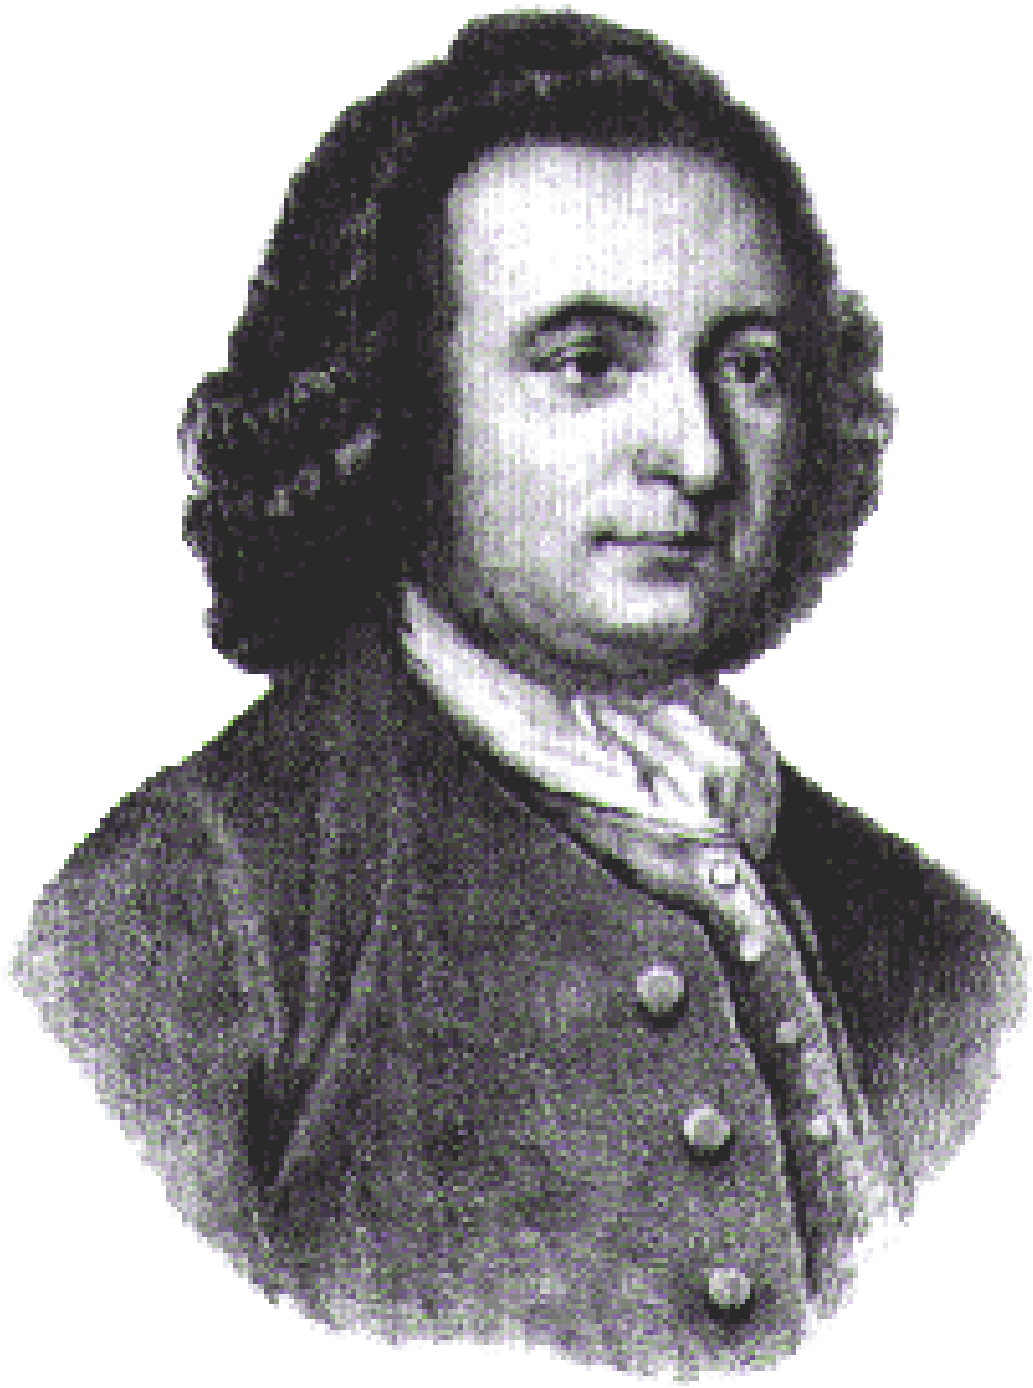
\includegraphics[width=0.5\linewidth,keepaspectratio,
    alt={The George Mason University seal.}]
    {figures/figGeorgeMason.pdf}
  \caption[The George Mason University seal]
  {The George Mason University seal, the example figure supplied with the UDTS template. Describe what the figure shows and name the source of the image.}
  \label{fig:example:mason}
\end{figure}

\section{A table}
\label{sec:example:table}

The caption of a table sits above it. The \verb|\tagpdfsetup| line marks the header row so the PDF records the table structure. Table~\ref{tab:example:values} gives example values.

\begin{table}[htbp]
  \centering
  \caption[Example values by case]
  {Example values by case. Units are in the column headings.}
  \label{tab:example:values}
  \tagpdfsetup{table/header-rows={1}}
  \begin{tabular}{lrr}
    \hline
    Case & Voltage (V) & Current (A) \\
    \hline
    A & 120 & 2.0 \\
    B & 240 & 1.5 \\
    C & 480 & 0.8 \\
    \hline
  \end{tabular}
\end{table}

\section{Equations}
\label{sec:example:equation}

Equations are numbered by chapter. The sentence after an equation defines every symbol in it. Ohm's law relates voltage, current, and resistance,
\begin{equation}
  V = I R,
  \label{eq:example:ohm}
\end{equation}
where $V$ is the voltage in volts, $I$ the current in amperes, and $R$ the resistance in ohms. The sample mean of $n$ observations is
\begin{equation}
  \bar{x} = \frac{1}{n} \sum_{i=1}^{n} x_i,
  \label{eq:example:mean}
\end{equation}
where $x_i$ is the $i$th observation. Both equations appear in the List of Equations through their labels.

\chapterreferences

\chapter{A Second Chapter}
\label{ch:second}

Each chapter ends with \verb|\chapterreferences|. In manuscript style it starts a new page, adds a References entry to the table of contents, and prints the works cited in that chapter. This chapter cites one work \cite{bor_revisiting_2026}, so its list has one entry. In traditional style the command prints nothing and one list follows the appendices.

\section{Headings}
\label{sec:second:headings}

Chapters are numbered as ``1.'' and sections as ``1.1'' in the template style. The headings are recorded as PDF headings for assistive technology. Use \verb|\chapter|, \verb|\section|, and \verb|\subsection| as in any LaTeX document.

\subsection{Cross references}
\label{sec:second:refs}

Refer to chapters, sections, figures, tables, and equations with \verb|\ref| and the kind spelled out: Chapter~\ref{ch:example}, Figure~\ref{fig:example:mason}, Table~\ref{tab:example:values}, Equation~\ref{eq:example:ohm}, and Appendix~\ref{app:data}.

\chapterreferences


% Appendices. Delete these three lines if you have none.
\appendix
\appendixeqnumbering
% An appendix starts with \appchapter instead of \chapter. The optional argument
% is the title shown in the table of contents.
\appchapter[Supplementary Data]{Supplementary Data}
\label{app:data}

Appendices follow the chapters and are lettered. Equations in an appendix are numbered with the appendix letter,
\begin{equation}
  a^2 + b^2 = c^2,
  \label{eq:appendix:pythagoras}
\end{equation}
where $a$ and $b$ are the legs of a right triangle and $c$ its hypotenuse.


% One reference list for the whole document, used when \referencelists is end.
\thesisreferences

\setlength{\parskip}{11pt}
\biography
Firstname M. Lastname received a Bachelor of Science from Name of University in 2019. Describe earlier study and work in one paragraph.

Describe the doctoral work, its funding, and any teaching or professional positions in a second paragraph.


\end{document}
